\section{Technische Umsetzung} \label{hannes}

\subsection{Datenaufbereitung}

\subsubsection{Herkunft und Umfang der Kursdaten}

\paragraph{Herkunft}
Die historischen Kursdaten der untersuchten Aktienticker werden über die Finanzplattform \textit{Yahoo Finance} \cite{yahoo} bezogen. Der Zugriff erfolgt über das Python-Paket \textit{yfinance} \cite{yfinance}, das die programmgesteuerte Abfrage von Open-High-Low-Close-Volume-(OHLCV)-Daten ermöglicht. \cite[S.~351]{mckinney_python_2018}, \cite{ismail_paper}

Um den Datensatz an verschiedene Untersuchungsszenarien anzupassen, wurde die Datenbeschaffung vollständig konfigurierbar gestaltet. Dies schließt unter anderem die Liste der betrachteten Ticker, den Zeitraum der Daten sowie das Zeitintervall der Kurse ein.

Für diese Untersuchung wurden Zeitreihen mit einer Länge von ca. acht Jahren verwendet, damit genügend Beobachtungspunkte vorlagen, um belastbare Aussagen über die Modellperformance unter verschiedenen Marktphasen treffen zu können.

\paragraph{Cache-Mechanismus}
Nach der programmgesteuerten Abfrage durch \textit{yfinance} werden die OHLCV-Daten in einem lokalen Cache gespeichert. Dies verkürzt die benötigte Zeit für wiederholte Durchläufe, da die Daten nicht mehr heruntergeladen werden müssen.

Die gespeicherten Daten sind ausschließlich rohe OHLCV-Daten. Jegliche Datenverarbeitung erfolgt bei jedem Durchlauf erneut, sodass Änderungen an der Konfiguration in einem neuen Durchlauf berücksichtigt werden.

\subsubsection{Feature-Engineering} \label{features}
Zur Datenverarbeitung gehört auch das Feature-Engineering, das auf Grundlage der rohen Daten zusätzliche Merkmale generiert. Dieser Schritt ist notwendig, da OHLCV-Daten nur in begrenztem Maße Strukturen aufweisen, die sich direkt modellieren lassen.

Ein zentrales Problem besteht in der Nichtstationarität der Aktienpreise. Diese folgen typischerweise keinem stationären Prozess, sondern lassen sich näherungsweise als Random Walk mit Drift modellieren. Dabei überlagert ein systematischer Trend die zufälligen Schwankungen der Zeitreihe:
\cite[S.~65]{tsay_analysis_2005}:
\begin{equation}
    p_t = \mu + p_{t-1} + \varepsilon_t
\end{equation}
Dabei bezeichnet $p_t$ den logarithmischen Preis zum Zeitpunkt $t$, $\mu$ den konstanten Drift und $\varepsilon_t$ das weiße Rauschen. Da sich der Mittelwert solcher Prozesse im Laufe der Zeit verändert,  würden klassische Machine-Learning-Modelle instabile Strukturen erlernen.
\cite[S.~64]{tsay_analysis_2005}

\paragraph{Logarithmische Renditen}
Finanzprozesse sind multiplikativer Natur, wodurch sich der einfache Preis $P_t$ zum Zeitpunkt $t$ durch \cite[S.~3]{tsay_analysis_2005}
\[
  P_t = P_{t-1} \cdot (1 + R_t)
\]
beschreiben lässt, wobei $R_t$ die einfache Rendite zwischen den Zeitpunkten $t-1$ und $t$ bezeichnet. Äquivalent gilt
\[
  R_t = \frac{P_t}{P_{t-1}}-1
\]
Da diese multiplikative Struktur statistisch schwer handhabbar ist, kann sie durch den natürlichen Logarithmus auch in additiver Form dargestellt werden \cite[S.~5]{tsay_analysis_2005}:
\begin{equation}
    r_t = \ln(1+R_t) = \ln \frac{P_t}{P_{t-1}} = p_t - p_{t-1}
\end{equation}
Daraus ergibt sich, dass die einfache Rendite $R_t$ die prozentuale Veränderung zweier einfacher Preise $P_t$ ist, während die logarithmische Rendite $r_t$ die Differenz zweier logarithmischer Preise $p_t$ ist.

\paragraph{Autoregression} \label{autoregression}
Lag-Features, auch verzögerte Variablen (lagged variables) genannt, repräsentieren die Vergangenheitswerte einer Zeitreihe und dienen dazu, serielle Abhängigkeiten wie Autokorrelation in einem Modell abzubilden. Ein Lag der Ordnung $k$ entspricht dem Wert einer Variable zum Zeitpunkt $t-k$. So entspricht etwa $r_{t-1}$ dem Lag 1. Ordnung der Rendite $r_t$.

Lag-Features bilden außerdem das Grundprinzip klassischer autoregressiver Modelle $AR(p)$. Dabei bezeichnet $p$ nicht den logarithmischen Preis, sondern die Ordnung des Modells. Für die Rendite $r_t$ ergibt sich ein autoregressives Modell der Ordnung $p$:
\begin{equation}
  r_t = \phi_0 + \phi_1r_{t-1} + \dots + \phi_pr_{t-p} + a_t 
\end{equation}

wobei $\phi_0$ eine Konstante, $\phi_1,\dots,\phi_p$ die Regressionskoeffizienten der jeweiligen Verzögerungen sind und $a_t$ den Effekt des weißen Rauschens darstellt. \cite[Kapitel 10.6]{fpp} \cite[S.~33]{tsay_analysis_2005}

In der Finanzmarktanalyse wird diese serielle Abhängigkeit oft als Momentum-Effekt interpretiert. Ein $AR$-Modell mit positiven Koeffizienten $(\phi>0)$ bildet hierbei die statistische Grundlage für den Momentum. Es beschreibt mathematisch, dass auf positive Renditen der Vergangenheit mit einer gewissen Wahrscheinlichkeit positive Renditen in der Gegenwart folgen. Durch die Einbeziehung mehrerer Lags kann das Modell komplexere Momentum-Muster über unterschiedliche Zeithorizonte hinweg erlernen.

Allerdings stellt die maximale Lag-Ordnung $p$, auch \texttt{max\_lag} im Programm genannt, eine zentrale Modellierungsentscheidung dar. Während eine größere Anzahl von Lags potenziell zusätzliche Informationen liefert, erhöht sie zugleich die Dimensionalität des Feature-Raums. Dies erhöht das Risiko von \textit{Overfitting}, bei dem ein Modell neben echten Zusammenhängen auch zufälliges Rauschen erlernt. Dadurch lernt das Modell Muster aus den historischen Daten, die im Testabschnitt nicht anwendbar sind. \cite[S.~220]{tesl} Abbildung~\ref{fig:complexity} zeigt, dass ein Overfit genau dort entsteht, wo der Prediction Error mit zunehmender Modellkomplexität wieder ansteigt. \cite[S.~220f.]{tesl}
\begin{figure}[H]
    \centering
    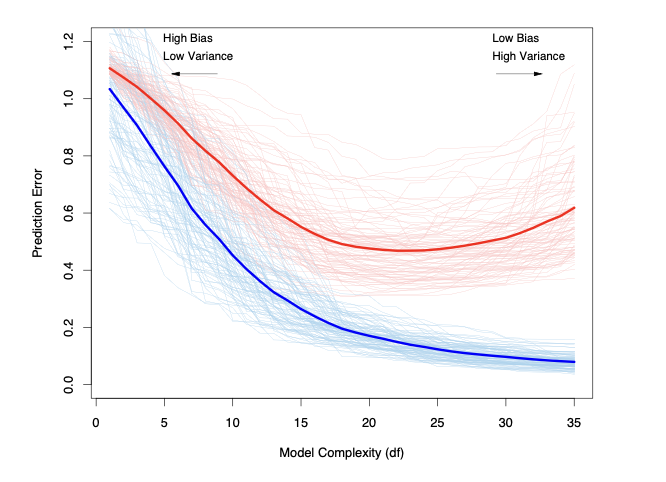
\includegraphics[width=0.8\textwidth]{images/complexity.png}
    \caption{Zusammenhang zwischen Modellkomplexität und \textit{Overfitting} \cite[S.~220]{tesl}}
    \label{fig:complexity}
\end{figure}

\paragraph{Rolling Fenster}
Zur Extraktion lokaler Trend- und Regimeinformationen werden sogenannte Rolling Features verwendet. Unter einem Marktregime versteht man einen Zeitabschnitt, in dem sich die statistischen Eigenschaften der Zeitreihe, wie z.B. Volatilität oder Trendrichtung, ähnlich verhalten und sich klar von anderen Phasen unterscheiden. Bei den Rolling Features werden statistische Daten über ein gleitendes Zeitfenster $w$ berechnet, das sich anschließend entlang der Zeitreihe verschiebt. Ziel dieser Transformation ist es, kurzfristige Schwankungen zu glätten und zugleich lokale Strukturen im Modell sichtbar zu machen. \cite[S.~354f.]{mckinney_python_2018}

Im Programm werden für jedes definierte Fenster $w \in \{5,10,20\}$ folgende Merkmale generiert:
\begin{itemize}
  \item \texttt{rolling\_mean\_w} bildet einen gleitenden Mittelwert des Schlusskurses ab und dient als Indikator für das lokale Preisniveau bzw. kurzfristige Trendrichtung. \cite[S.~355]{mckinney_python_2018}
  \item \texttt{rolling\_std\_w} berechnet eine gleitende Standardabweichung und dient als Maß für die kurzfristige Volatilität. \cite[S.~356]{mckinney_python_2018}
  \item \texttt{rolling\_min\_w} und \texttt{rolling\_max\_w} bilden lokale Extremwerte ab und liefern Informationen über Range-Strukturen sowie mögliche Breakout-Situationen. \cite[S.~160]{mckinney_python_2018}
\end{itemize}

Die Effekte dieser Features werden in Abb.~\ref{fig:rolling} visualisiert. Der Einbruch Anfang 2025 zeigt exemplarisch, wie die rollende Standardabweichung erhöhte Marktvolatilität erfasst, während Minimum und Maximum die lokale Preisspanne abbilden.
\begin{figure}[H]
    \centering
    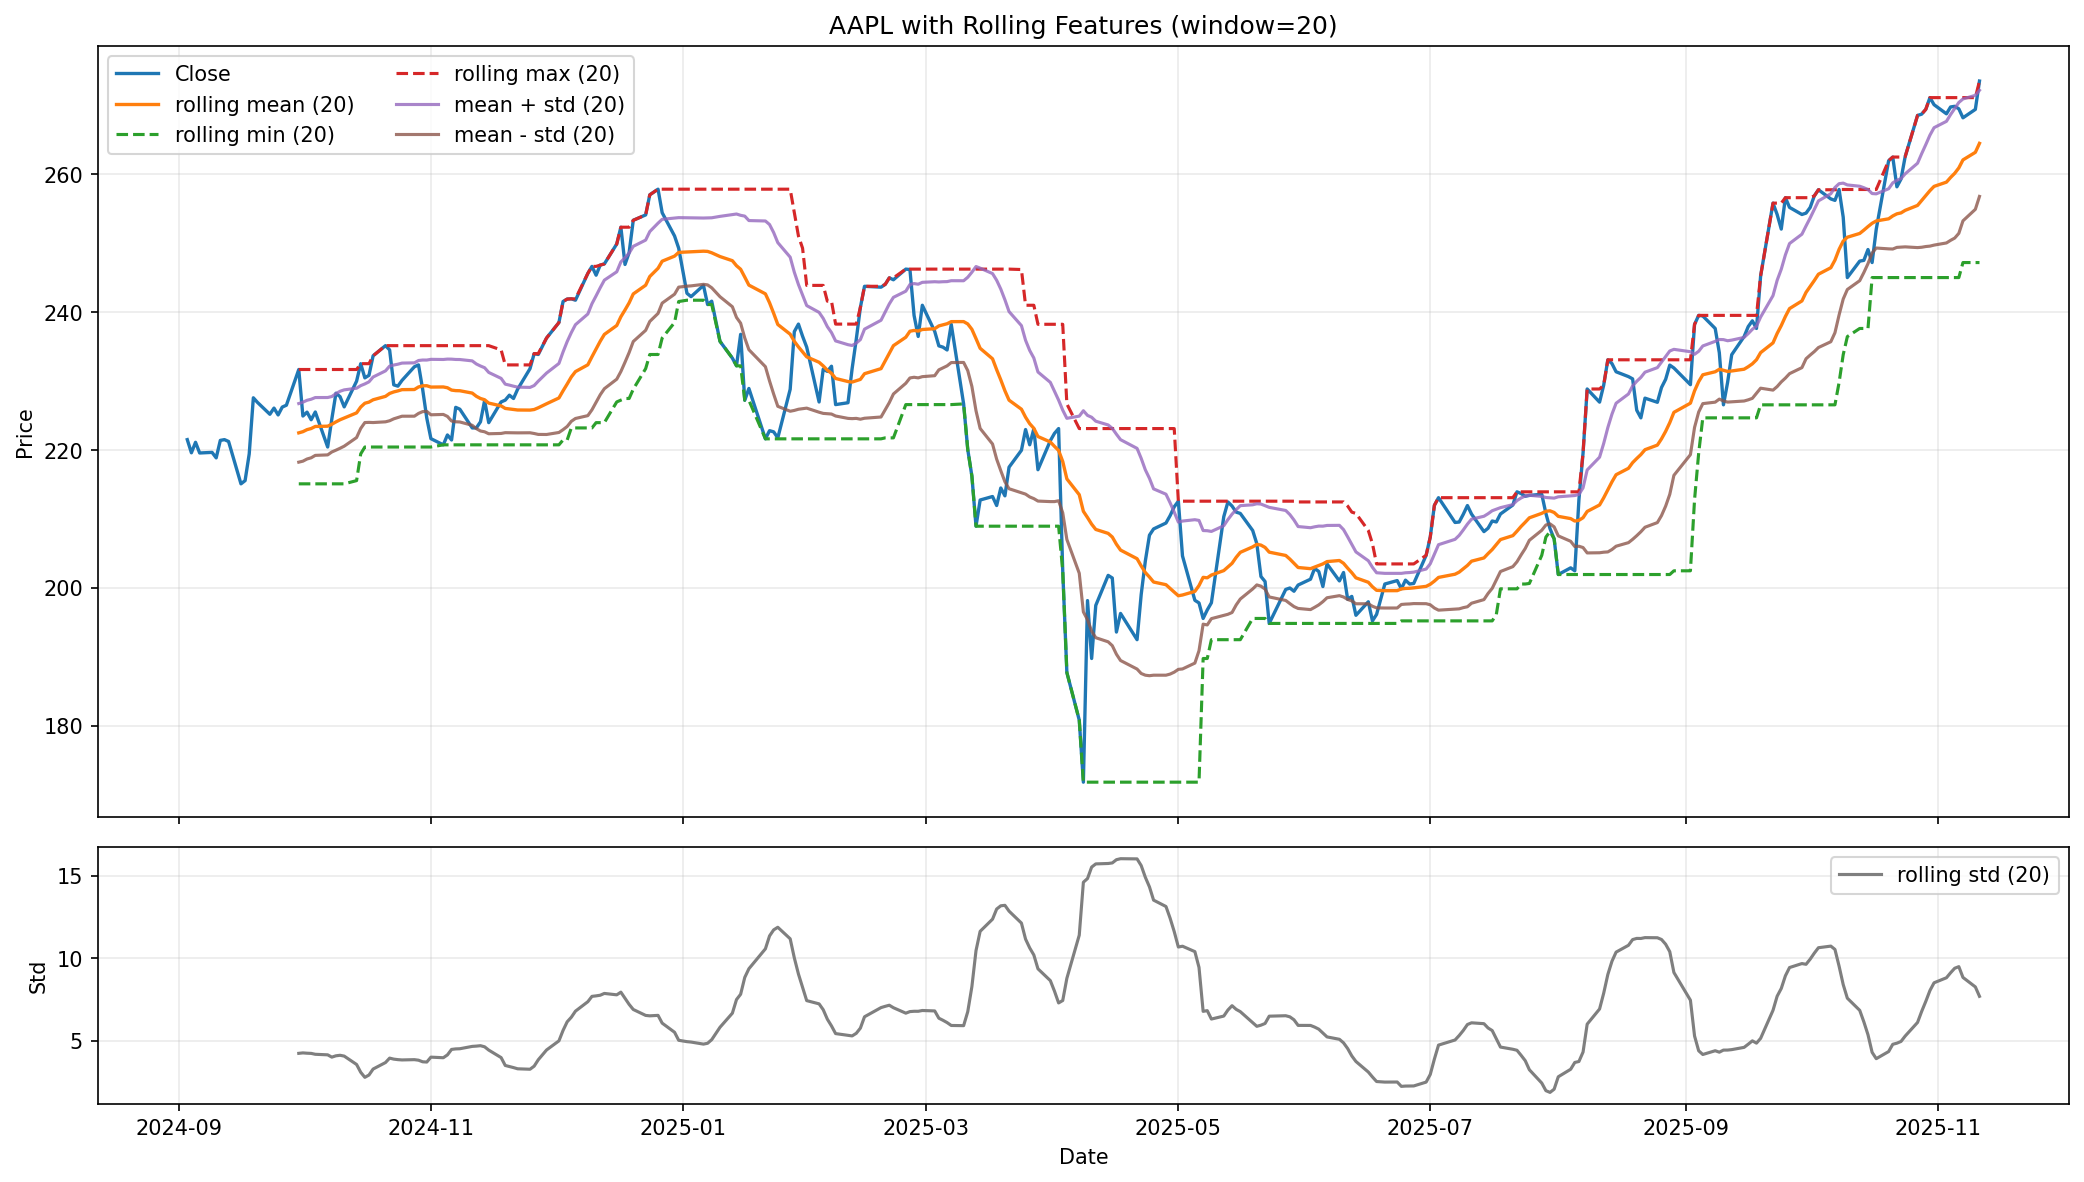
\includegraphics[width=0.8\textwidth]{images/rolling.png}
    \caption[Visualisierung von Rolling-Features]{Visualisierung der Rolling-Features für den DIA ETF mit einer Fenstergröße von $w=20$}
    \label{fig:rolling}
\end{figure}
Die Rolling-Features werden mithilfe des \textit{rolling}-Operators der Python Bibliothek \textit{pandas} \cite{pandas} sowie Aggregationsfunktionen wie \texttt{mean()}, \texttt{std()}, \texttt{min()} und \texttt{max()} erzeugt. Die Wahl der Fenstergröße $w$ unterliegt einem klassischen Bias-Varianz-Tradeoff, denn während kleinere Fenster schneller reagieren, sind sie auch anfälliger für Rauschen.

\paragraph{Volatilitäts- und Marktaktivitätsmetriken}
Auch Volatilität und Marktvolumen werden als Features in die Modelle integriert, um verschiedene Marktregime zu quantifizieren. Volatilität beschreibt den Schwankungsbereich von Kursen und damit auch das Risikoniveau, während das Marktvolumen, das in den OHLCV enthalten ist, die allgemeine Marktaktivität darstellt. \cite[S.~22]{wilder_new_1978}

Die im Programm eingesetzten Volatilitätsmaße basieren entweder auf bereits vorhandenen Rolling-Features wie der Standardabweichung \texttt{rolling\_std\_w} oder auf der von J.~Welles Wilder entwickelten Average True Range (ATR). Zunächst wird für jeden Handelstag die sogenannte True Range (TR) definiert:
\begin{equation}
  \text{TR}_t = \max \left\{
  \begin{aligned}
    & H_t - L_t, \\
    & |H_t - C_{t-1}|, \\
    & |L_t - C_{t-1}|
  \end{aligned}
  \right\}
\end{equation}
wobei $H_t$ das Tageshoch, $L_t$ das Tagestief und
$C_{t-1}$ ist der Schlusskurs des Vortages. \cite[S.~21]{wilder_new_1978} Durch diese Definition werden auch Kurslücken zwischen zwei Handelstagen berücksichtigt, wodurch die True Range ein robusteres Schwankungsmaß darstellt als die reine Intraday-Spanne. Anschließend wird der ATR als gleitender Mittelwert der True Range bestimmt:
\begin{equation}
  \mathrm{ATR}_t^{(w)} = \frac{1}{w}\sum_{i=0}^{w-1}\mathrm{TR}_{t-i}.
\end{equation}
\cite[S.~23]{wilder_new_1978}, wobei $w$, im Programm \texttt{vol\_window}, der Fenstergröße entspricht.

\subsubsection{Split-Strategie sowie Skalierungs- und Zielgenerierung}

\paragraph{Split-Strategie}
Bevor diese Features in die Modelle einfließen können, muss der Datensatz so aufgeteilt werden, dass die Generalisierungsfähigkeit der Modelle evaluiert werden kann. Dabei wird das Datenset in Trainings-, Validierungs- und Testabschnitte aufgeteilt. Die Split-Strategie soll außerdem die Entstehung von \textit{Lookahead-Bias} und \textit{Overfitting} vermeiden. Ein Lookahead-Bias entsteht durch sogenanntes \textit{Data Leakage}, also wenn Informationen aus einem zeitlich späteren Abschnitt in den Trainingsprozess einfließen, die in der Realität zum jeweiligen Zeitpunkt noch nicht vorgelegen hätten. \cite[S.~222]{tesl}

\paragraph{Skalierung}
Für bestimmte Modelle, insbesondere die Ridge Regression, müssen die Features standardisiert werden, da lineare Algorithmen sehr empfindlich auf unterschiedliche Skalierungen bei den Inputs reagieren. Baumbasierte Modelle wie der Random Forest sind hingegen skaleninvariant, profitieren jedoch von einer einheitlichen Datenvorverarbeitung. Die Features werden so transformiert, dass sie einen Mittelwert von Null und eine Einheitsvarianz (Standardabweichung von 1) haben. \cite[S.~604]{tesl} Dabei ist es entscheidend, dass diese Transformationen ausschließlich auf Basis des Trainingsabschnitts berechnet werden, um sicherzustellen, dass keine Informationen aus der Zukunft, also Daten aus den Validierungs- und Testabschnitten, in das Training einfließen. \cite[S.~389]{mckinney_python_2018}

\paragraph{Zielgenerierung}
Für jeden Horizont werden genau zwei Ziele generiert: das Regressionsziel und das Klassifikationsziel.

Während das Regressionsziel einen numerischen Wert darstellt, konkret eine volatilitätsskalierte zukünftige Log-Rendite, zielt das Klassifikationsziel darauf ab, eine binäre Dummy-Variable zu bestimmen, die angibt, ob der Kurs im jeweiligen Horizont steigen oder sinken wird. \cite[S.~10]{tesl}

\subsection{Modellierung}
\subsubsection{Regressionsmodelle} \label{regression}
Mit den aufbereiteten, aufgeteilten und skalierten Daten können nun die verschiedenen Modellarchitekturen trainiert werden. Darunter auch die Regression, die im maschinellen Lernen eine Variante des überwachten Lernens (Supervised Learning) ist. Das Ziel der Regression ist, eine Ausgangs- oder abhängige Variable $Y$ vorherzusagen. \cite[S.~10]{tesl}

Lineare Regression (LR) dient als Ausgangspunkt für den Vergleich weiterer Regressionsmodelle. Sie basiert auf der Annahme eines linearen Zusammenhangs zwischen der Zielvariable und den Eingangsvariablen. Das Modell beschreibt diese Zielvariable als gewichtete Summe der Features:
% Formel 3.1 + 2.1
\begin{equation}
  \hat{f}(X) = \hat{\beta}_0 + \sum_{j=1}^{p}X_j\hat{\beta}_j
\end{equation}
Dabei bezeichnet $\hat{\beta}_j$ den geschätzten Einfluss des jeweiligen Features $X_j$ auf die Zielvariable \cite[S.~11,44]{tesl}. Wenn man dies spezifisch auf das additive Fehlermodell bezieht, entsteht der Zusammenhang:
%Formel 2.29
\begin{equation}
  Y = f(X) + \varepsilon
\end{equation}
wobei $\varepsilon$ den zufälligen Fehlerterm repräsentiert. \cite[S.~28]{tesl} Durch diesen Fehlerterm entsteht eine Differenz zwischen beobachtetem $y_i$ und vorhergesagtem $\hat{y}_i$ Wert, welche als Residuum $e_i=y_i-\hat{y}_i$ bezeichnet wird. Aus diesem Residuum wird in der Statistik die Fehlerfunktion Residual Sum of Squares (RSS) berechnet:
\begin{equation} \label{rss}
  \text{RSS} = \sum_{i=1}^{N} (y_i - \hat{y}_i)^2
\end{equation}
Durch das Quadrieren werden die Fehler immer positiv und größere Fehler stärker gewichtet. Dadurch misst die RSS das \glqq Lack of Fit\grqq{}, also wie schlecht das Modell zu den Daten passt. \cite[S.~12]{tesl}

Durch ihre mathematische Einfachheit bringt sie auch strukturelle Nachteile mit sich. Lineare Regression wird bei hoher Dimensionalität instabil, wenn die Anzahl der generierten Features $p$ größer ist als die Anzahl der Datenpunkte $N$ ($p>N$). Außerdem neigt LR in solchen hochdimensionalen Szenarien zu hoher Varianz. Das bedeutet, dass schon kleine Unterschiede in den Trainingsdaten zu erheblichen Änderungen der Koeffizienten des Modells und damit zu Overfitting führen. \cite[S.~47,649]{tesl}

\paragraph{Ridge Regression} \label{ridge}
Die Ridge Regression (RR) ist eine Erweiterung der klassischen linearen Regression, die in hochdimensionalen Szenarien ($p \gg N$) deutlich stabiler ist. Dies wird durch das Hinzufügen eines Strafterms (Penalty Term) zur Fehlerfunktion RSS aus der Formel \ref{rss} umgesetzt. In der Statistik wird dieses erweiterte Kriterium als Penalized Residual Sum of Squares (PRSS) bezeichnet. Die allgemeine Struktur lautet:
%Formel 2.38
\begin{equation}
  \text{PRSS}(f; \lambda) = \text{RSS}(f) + \lambda J(f)
\end{equation} \cite[S.~34]{tesl} wobei $J(f)$ die mathematische Bestrafung der Modellkomplexität und $\lambda$ den Regularisierungsparameter, der die Stärke der Bestrafung bestimmt, darstellen. Bei der Ridge Regression wird als Strafterm $J(f)$ der sogenannte \textit{L2-Penalty} verwendet, der die Summe der quadrierten Koeffizienten der Features darstellt. Dieser bestraft große Koeffizientenwerte, wodurch das Modell gezwungen wird, den Einfluss einzelner Features zu 
begrenzen. Die optimalen Koeffizienten $\hat{\beta}_{\text{ridge}}$ der Features des Modells ergeben sich durch die Minimierung der folgenden Funktion:
%Formel 3.41
\begin{equation} 
  \hat{\beta}_{\text{ridge}} = \underset{\beta}{\text{argmin}} \left\{\sum_{i=1}^{N} \left( y_i - \beta_0 - \sum_{j=1}^{p} x_{ij}\beta_j \right)^2 + \lambda \sum_{j=1}^{p} \beta_j^2 \right\}
\end{equation} 
\cite[S.~62]{tesl}

Hierbei ist $\lambda$ ein Komplexitätsparameter, der die Stärke der Schrumpfung kontrolliert: Je größer der Wert von $\lambda$, desto stärker wird das Modell gezwungen, die Koeffizienten in Richtung $0$ zu schrumpfen (Shrinkage). Dadurch wird erreicht, dass kein Feature das gesamte Modell dominiert. Dabei entsteht zwar ein Verlust an Genauigkeit gegenüber den Trainingsdaten (Bias), allerdings lernt das Modell weniger Rauschen (Varianz) und wird damit für neue Daten vorhersagekräftiger. \cite[S.~63f.]{tesl}

\paragraph{Random Forest} \label{rf}
Random Forest ist ein \textit{Ensemble}-Modell, das auf dem Prinzip des \textit{Bagging} (Bootstrap Aggregation) basiert. Dabei werden mehrere Entscheidungsbäume jeweils auf einer zufälligen Teilmenge der Trainingsdaten (Bootstrap-Stichprobe) trainiert und ihre Vorhersagen anschließend gemittelt, wodurch die hohe Varianz einzelner Bäume reduziert wird. Diese Architektur ist in 
Abbildung~\ref{fig:rf} schematisch dargestellt.
\begin{figure}[H]
    \centering
    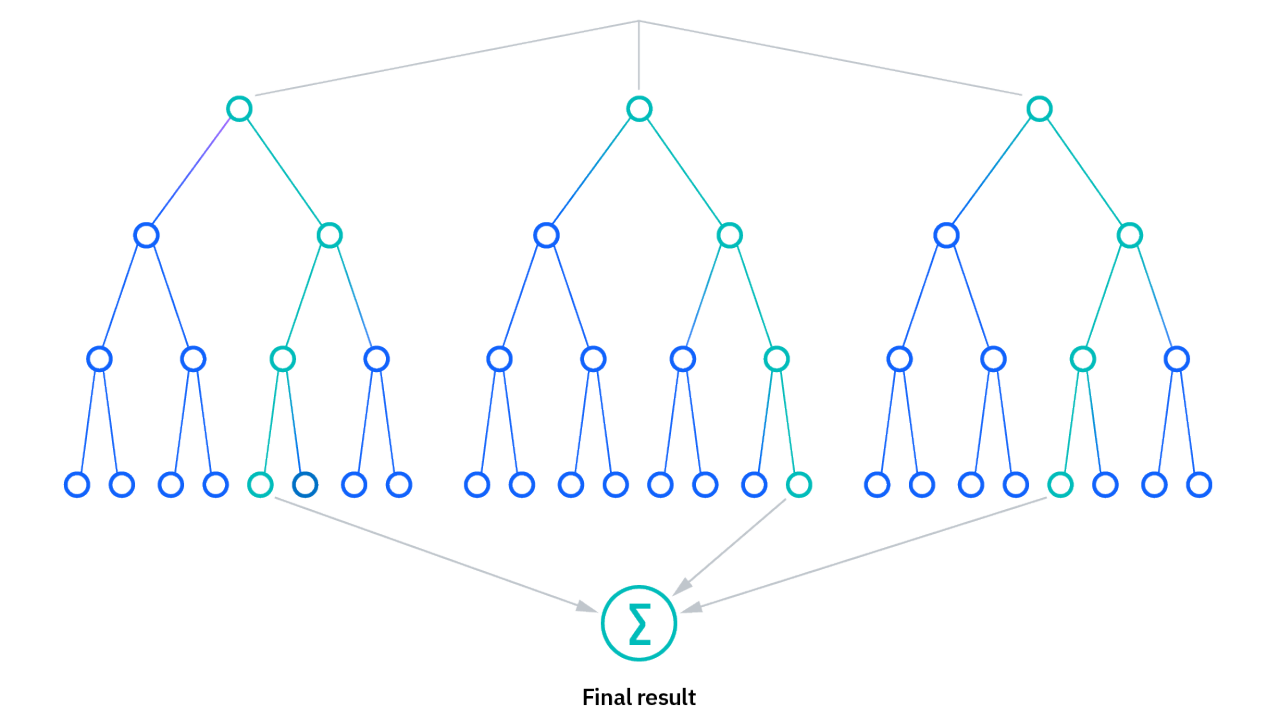
\includegraphics[width=0.8\textwidth]{images/rf.png}
    \caption{Visualisierung eines Random Forests \cite{ibm}}
    \label{fig:rf}
\end{figure}
Ein Problem des klassischen Baggings besteht darin, dass die verschiedenen Bäume, trotz unterschiedlicher Stichproben, aufgrund stark gewichteter Features stark korreliert bleiben. Der Random Forest behebt dieses Problem durch eine zusätzliche Zufälligkeitsebene, da bei einer Entscheidung nicht mehr alle Features $p$ berücksichtigt werden, sondern nur eine zufällige Teilmenge von $m$ Features. In der Literatur wird bei Regressionsanwendungen diese Teilmenge oft auf $m=\frac{p}{3}$ festgelegt. \cite[S.~592]{tesl}

Im Gegensatz zu linearen Modellen wie der Ridge Regression setzt der Random Forest keinen linearen Zusammenhang zwischen den Features und der Zielvariable voraus, weshalb dieses Modell auch nichtlineare Strukturen in den Daten lernt. Gegenüber linearen Modellen hat der Random Forest den zusätzlichen Vorteil, dass er in hochdimensionalen Szenarien weniger zum \textit{Overfitting} neigt. \cite[S.~587f.]{tesl}

\subsubsection{Richtungsklassifikatoren} \label{logistic}
Neben der Renditeprognose wird im Programm zusätzlich eine Richtungsklassifikation implementiert, um die Bewegung einer Aktie vorherzusagen. Im Gegensatz zur Regression wird kein numerischer Wert, sondern eine binäre Einschätzung vorhergesagt, ob sich die Aktie nach unten oder nach oben bewegen wird. \cite[S.~10]{tesl}

\paragraph{Logistische Regression} \label{logistical_regression}
Als Grundlagenmodell wird die logistische Regression verwendet, ein Standardverfahren des überwachten Lernens für binäre Klassifikationen \cite{ismail_paper}. Sie modelliert die bedingte Wahrscheinlichkeit $Pr(G = k \mid X = x)$, also die Wahrscheinlichkeit, dass ein Beobachtungspunkt mit den Features $x$ einer bestimmten Klasse zugeordnet wird. Namensgebend ist die sogenannte Logit-Transformation, die die Gewinnchance (Odds) $\frac{p}{1-p}$ logarithmiert (Log-Odds). \cite[S.~102]{tesl} Diese lässt sich umformen zur Sigmoid-Funktion 
\begin{equation}
    \sigma(z) = \frac{1}{1 + e^{-z}} = \frac{e^z}{1 + e^z}
\end{equation}
umgeformen, welche die Wahrscheinlichkeit $Pr(G = k \mid X = x)$ als
\begin{equation}
    \Pr(G=1 \mid X=x) = \frac{e^{\beta_0 + \beta^T x}}{1 + e^{\beta_0 + \beta^T x}}
\end{equation}
beschreibt. \cite[S.~102]{tesl} Durch diese Transformation wird sichergestellt, dass die Modellvorhersagen immer den gesamten reellen Zahlenraum $\mathbb{R} = (-\infty,+\infty)$ abdecken, im Intervall $[0,1]$ liegen und somit mathematisch als Wahrscheinlichkeiten betrachtet werden können. \cite[S.~119f.]{tesl}

\paragraph{Meta-Klassifikator}
Um die Richtungsprognose zu verbessern, wird die logistische Regression als Meta-Learner eingesetzt. Dabei werden beim \textit{Stacking} die Vorhersagen verschiedener Modelle 
als zusätzliche Features für ein übergeordnetes Modell, den Meta-Learner, verwendet \cite[S.~290]{tesl}. Die Stärke eines Meta-Modells liegt darin, dass es die Stärken verschiedener Modellarchitekturen vereint und dadurch die Varianz der Vorhersagen sowie den Gesamtfehler reduziert \cite{ismail_paper}. Lineare Modelle wie die Ridge Regression (Abschnitt~\ref{ridge}) erfassen stabile Trends, während nichtlineare Modelle wie der Random Forest (Abschnitt~\ref{rf}) besonders komplexe Zusammenhänge zwischen Features modellieren können. Zusätzlich fließen auch die regulären Features sowie ARIMA-Signale (\ref{arima}) in die Vorhersage des Meta-Learners mit ein.

\paragraph{Referenzlinie}
Um die Modellleistung der beiden Klassifikationsmodelle objektiv miteinander zu vergleichen, wird zusätzlich ein naiver Referenzwert definiert. In diesem Fall wird die sogenannte Base Error Rate als Referenz verwendet. Sie beschreibt den Fehler, der entsteht, wenn ausschließlich der 
Der Mittelwert der Trainingsdaten wird als Vorhersage verwendet. Dadurch liegt die ausgegebene Wahrscheinlichkeit $Pr(G = k \mid X = x)$ bei einer binären Richtungsklassifikation immer am historischen Mittelwert der Trainingsdaten, weshalb dieses Modell die reine Klassenhäufigkeit darstellt. \cite[S.~51]{tesl}

\subsubsection{Autoregressive Integrated Moving-Average Modelle}
\label{arima}
Neben den machine-learning-basierten Ansätzen wird als Vergleich ein klassisches Zeitreihenmodell (ARIMA) eingesetzt. Ein ARIMA-Modell ist ein autoregressives, integriertes, gleitendes Durchschnittsmodell, das als Erweiterung der ARMA-Modelle für nicht-stationäre Zeitreihen entwickelt wurde \cite[S.~67f.]{tsay_analysis_2005} und aus drei Komponenten besteht:
\begin{itemize}
    \item \textbf{Autoregression (AR)} beschreibt die Abhängigkeit einer Variable von ihren eigenen historischen Werten.
    \item \textbf{Integration (I)} bezeichnet das Differenzieren der Daten, um Stationarität zu erreichen. Ein Prozess ist $I(1)$, wenn seine ersten Differenzen stationär sind, was bei Aktienpreisen häufig der Fall ist.
    \item \textbf{Moving Average (MA)} modelliert die Abhängigkeit der Variable von den vergangenen Vorhersagefehlern (Schocks).
\end{itemize}
Ein $\mathrm{ARIMA}(p,d,q)$ Modell lässt sich mithilfe der Backshift-Notation 
mathematisch wie folgt darstellen: \cite[Formel 9.2]{fpp}
\begin{equation}
    (1 - \phi_1 B - \cdots - \phi_p B^p)(1-B)^d y_t = c + (1 + \theta_1 B + \cdots + \theta_q B^q)\varepsilon_t
\end{equation}
Dabei verschiebt der Backshift-Operator $B$ die Zeitreihe um einen Schritt in die Vergangenheit, d.h. $B y_t = y_{t-1}$. Der linke Klammerausdruck $(1 - \phi_1 B - \cdots - \phi_p B^p)$ beschreibt die AR-Komponente mit den 
Koeffizienten $\phi_i$, während $(1-B)^d$ die $d$-fache Differenzierung der Zeitreihe darstellt. Auf der rechten Seite enthält $(1 + \theta_1 B + \cdots + \theta_q B^q)$ die MA-Komponente mit den Koeffizienten $\theta_1 , \cdots , \theta_q$ und den Weißrauschprozess $\varepsilon_t$. Ein besonderes Merkmal von ARIMA-Prozessen ist ihr starkes Gedächtnis, denn sogenannte Schocks wirken sich dauerhaft auf den Prozess aus, da sie nicht ausgedämpft werden. Die optimale Modellordnung $(p, d, q)$ wird im Programm mittels Grid-Search nach dem niedrigsten Akaike-Informationskriterium (AIC) bestimmt. Das AIC bewertet Modelle anhand ihrer Anpassungsgüte und bestraft zugleich eine höhere Modellkomplexität. \cite[Kapitel 9.5,9.6]{fpp}

\paragraph{Saisonalität}
Das saisonale Erweiterungsmodell $\mathrm{SARIMA}(p,d,q)(P,D,Q)_m$ ergänzt das klassische ARIMA um eine saisonale Komponente mit der Periode $m$, wobei $m$ die Anzahl der Beobachtungen pro Saison angibt. Großbuchstaben bezeichnen dabei die saisonalen Parameter, Kleinbuchstaben die nicht-saisonalen.

Die saisonalen Terme sind analog zu den nicht-saisonalen Komponenten aufgebaut, verwenden jedoch Backshifts der saisonalen Periode $m$ statt einfacher Backshifts. Beide Teile werden miteinander multiplikativ verknüpft. Ein $\mathrm{SARIMA}(1,1,1)(1,1,1)_4$ Modell für Quartalsdaten ($m=4$) lässt sich beispielsweise wie folgt darstellen:
\begin{equation}
    (1-\phi_1 B)(1-\Phi_1 B^4)(1-B)(1-B^4)y_t = (1+\theta_1 B)(1+\Theta_1 B^4)\varepsilon_t
\end{equation}
Dabei bezeichnen $\Phi_1$ und $\Theta_1$ die saisonalen Gegenstücke zu den nicht-saisonalen Koeffizienten $\phi_1$ und $\theta_1$. Die saisonale Struktur eines Modells lässt sich anhand der Autokorrelationsfunktion (ACF) und der partiellen Autokorrelationsfunktion (PACF) identifizieren, da die saisonalen AR- und MA-Terme bei den saisonalen Lags sichtbar werden. Für diese Untersuchung wird die saisonale Periode im Programm auf $m = 5$ Handelstage festgelegt, um wöchentliche Muster in den Kursdaten zu erfassen \cite[Kapitel 9.9]{fpp}.

\subsubsection{Deep Learning Modelle}
Während ARIMA auf linearen Abhängigkeiten basiert, ermöglichen Deep-Learning-Modelle die Abbildung komplexer und nichtlinearer Muster in Zeitreihen. Deep Learning basiert auf künstlichen neuronalen Netzen (Artificial Neural Networks, ANN), die als nichtlineare Modelle betrachtet werden können. Ein klassisches Feed-Forward-Netz besteht aus einer Eingabeebene (Input Layer), versteckten Ebenen (Hidden Layers) und einer Ausgabeebene (Output Layer), wie in Abbildung~\ref{fig:feed_forward} dargestellt.
\begin{figure}[H]
    \centering
    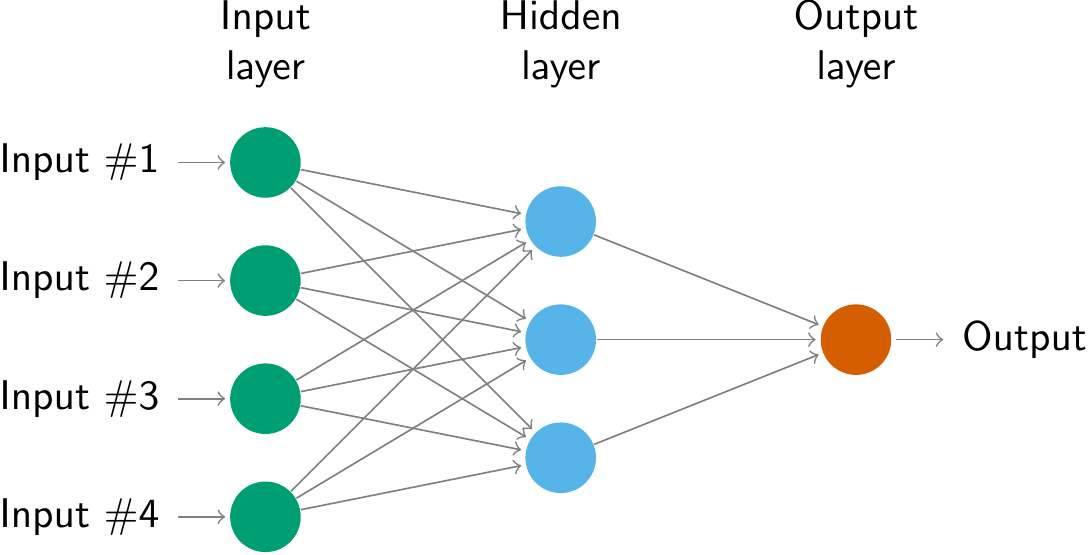
\includegraphics[width=0.8\textwidth]{images/feed_forward.png}
    \caption{Visualisierung der Ebenen eines Feed-Forward-Netzes \cite[Kapitel 12.4]{fpp}}
    \label{fig:feed_forward}
\end{figure}
Die Nichtlinearität wird durch eine Aktivierungsfunktion erzeugt. Häufig wird dafür die Sigmoid-Funktion (Abschnitt \ref{logistical_regression}) verwendet, um die Ausgabe auf das Intervall $[0,1]$ zu begrenzen. \cite[S.~392f.]{tesl}

\paragraph{Long Short-Term Memory Modelle} Während einfache Feed-Forward-Netze Schwierigkeiten haben, sequentielle Abhängigkeiten in Finanzzeitreihen abzubilden, können rekurrente Architekturen wie Long Short-Term Memory (LSTM)-Netze diese zeitlichen Zusammenhänge lernen. Ihre Besonderheit liegt in der Fähigkeit, auch langfristige Abhängigkeiten in den Daten zu identifizieren. Kayit und Ismail \cite{ismail_paper} belegen zudem, dass LSTMs tägliche Aktienkurse präziser vorhersagen können als traditionelle Machine-Learning-Modelle, was ihre Eignung für Finanzzeitreihen unterstreicht \cite{hochreiter_long_1997}. 

\subsection{Evaluierung}

\subsubsection{Versuchsaufbau}

Um die Leistung der behandelten Modelle objektiv beurteilen zu können, wird ein einheitlicher Versuchsrahmen festgelegt. Als Datenbasis dienen vier börsengehandelte Indexfonds (SPY, QQQ, DIA, XLE) mit insgesamt ca. 2.035 Handelstagen im Zeitraum von Januar 2018 bis Februar 2026. \cite{ismail_paper} Die Daten werden chronologisch in Trainings- (70\,\%), Validierungs- (15\,\%) und Testabschnitt (15\,\%, ca. 300 Beobachtungen) aufgeteilt, sodass kein Lookahead-Bias entstehen kann. \cite[S.~222]{tesl}

Für die Regressionsmodelle werden folgende Metriken als Fehlermaße verwendet:
\begin{itemize}
    \item \texttt{Root Mean Squared Error (RMSE)} misst den mittleren quadratischen Abstand zwischen Vorhersage und tatsächlichem Wert und wichtet daher große Fehler stärker. \cite[Kapitel 5.8]{fpp}
    \item \texttt{Mean Absolute Error (MAE)} misst den durchschnittlichen absoluten Abstand zwischen Vorhersage und tatsächlichem Wert. \cite[Kapitel 5.8]{fpp}
    \item \texttt{symmetric Mean Absolute Percentage Error (sMAPE)}, der den prozentualen Fehler relativ zur Größe der Werte misst und dabei symmetrisch für Über- und Unterschätzungen ist. \cite[Kapitel 5.8]{fpp}
    \item \texttt{Bestimmtheitsmaß $R^2$}, das misst, wie viel besser das Modell im Vergleich zur Null-Baseline abschneidet, wobei $R^2 = 1$ einer perfekten Vorhersage und $R^2 < 0$ einer schlechteren Vorhersage als die Null-Baseline entspricht. \cite[Kapitel 7.2]{fpp}
    \item \texttt{Richtungsgenauigkeit (Directional Accuracy)} misst den Anteil der Beobachtungen, bei denen das Modell die Bewegungsrichtung korrekt vorhersagt.
\end{itemize}
Für die Klassifikation werden hingegen folgende Maße verwendet:
\begin{itemize}
    \item \texttt{Accuracy}, der Anteil der korrekt klassifizierten Beobachtungen an allen Beobachtungen.
    \item \texttt{F1-Score}, welcher das harmonische Mittel aus Precision und Recall darstellt und damit sowohl falsch-positive als auch falsch-negative Vorhersagen berücksichtigt. \cite{ismail_paper}
    \item \texttt{Receiver Operating Characteristic - Area Under the Curve (ROC-AUC)} misst die Fläche unter der Receiver-Operating-Characteristic-Kurve und bewertet die Trennfähigkeit des Modells zwischen den Klassen unabhängig vom gewählten Schwellenwert. \cite{ismail_paper}
    \item \texttt{Brier-Score}, der den mittleren quadratischen Abstand zwischen den vorhergesagten Wahrscheinlichkeiten und den tatsächlichen Klassen misst, wobei ein niedriger Wert auf eine bessere Kalibrierung hindeutet.
    \item \texttt{Coverage}, der den Anteil der Beobachtungen misst, für die das Modell überhaupt eine binäre Vorhersage trifft.
\end{itemize}

Als Vergleichsbaselines dienen zwei naive Referenzmodelle. Einmal \texttt{zero\_return}, das stets eine Rendite von null prognostiziert, sowie \texttt{baseline\_rate}, das stets die Trainings-Basisrate als Klassenwahrscheinlichkeit ausgibt.

\subsubsection{Regressionsergebnisse}

\begin{table}[ht]
\centering
\caption{Regressionsmetriken aus dem Testset ($h = 5$ Handelstage)}
\label{tab:regression_h5}

\begin{tabularx}{\linewidth}{llRRRRR}
\toprule
\textbf{Ticker} & \textbf{Modell} & \textbf{RMSE} & \textbf{MAE} & \textbf{sMAPE\,(\%)}$^\dagger$ & \textbf{$R^2$} & \textbf{Dir.\ Acc.} \\
\midrule
  \multirow{4}{*}{\textbf{DIA}} & Ridge & 1.646 & 1.424 & 75.9 & $-$1.354 & 0.423 \\
   & Random Forest & 1.603 & 1.400 & \textcolor{bestgreen}{\textbf{75.9}} & $-$1.231 & 0.417 \\
   & SARIMA & \textcolor{bestgreen}{\textbf{1.075}} & \textcolor{bestgreen}{\textbf{0.811}} & 99.4 & \textcolor{bestgreen}{\textbf{$-$0.004}} & \textcolor{bestgreen}{\textbf{0.540}} \\
   & Zero-Return$^\ddagger$ & 1.076 & 0.811 & 100.0 & $-$0.005 & --- \\
\bottomrule
\end{tabularx}

\smallskip
{\footnotesize
$^\dagger$\,Skaliert mit Faktor $0{,}5$ (0--100\,\%) \quad $^\ddagger$\,Zero-Return: naive Baseline (Renditeprognose\,$= 0$). \quad
\textcolor{bestgreen}{\textbf{Grün}}: bestes Modell je Metrik.}
\end{table}

\paragraph{Vergleich der Modelle gegen die Null-Baseline}

Alle Modelle erzielen im Testabschnitt ein negatives $R^2$ und sind damit schlechter als eine triviale Nullprognose, die schlicht eine Rendite von null vorhersagt. Das gilt für alle getesteten Prognosehorizonte. Die gelernten Feature-Muster übertragen sich offenbar nicht auf neue Daten, was darauf hindeutet, dass die Modelle im Training Zufallsmuster aufgenommen haben, die im Testabschnitt nicht mehr vorhanden sind.

\paragraph{Richtungsgenauigkeit}
Bei der Richtungsgenauigkeit, also der Frage, ob das Modell wenigstens die Bewegungsrichtung korrekt vorhersagt, liegen die ML-Modelle durchgehend unter 50\,\% und schneiden damit schlechter ab als das zufällige Raten. SARIMA bildet hier eine Ausnahme. Bei einzelnen Ticker-Horizont-Kombinationen, wie $\mathrm{DIA}$ bei $h=5$, erreicht es eine Richtungsgenauigkeit von $0{,}540$ und damit knapp über 50\,\%. Außerdem erreicht es diesen Wert ohne Feature-Engineering. Das legt nahe, dass die vielen generierten Features eher Rauschen als nutzbare Informationen in die Prognose einbringen.

Wie in Abbildung~\ref{fig:regression} zu sehen ist, folgt die ARIMA-Prognose für DIA dem langfristigen Aufwärtstrend über den gesamten Testzeitraum hinweg eng. Trotz eines $R^2$ von $-0{,}004$ und einer Richtungsgenauigkeit von $0{,}540$ zeigt sich bei näherer Betrachtung, dass das Modell abrupte 
Kurskorrekturen, wie z.B. den Einbruch Mitte November 2025, kaum antizipiert. Die scheinbar gute visuelle Übereinstimmung ist damit kein Zeichen echter Vorhersagekraft, sondern ein Artefakt des zugrunde liegenden Aufwärtstrends, dem das Modell lediglich folgt.

\begin{figure}[H]
    \centering
    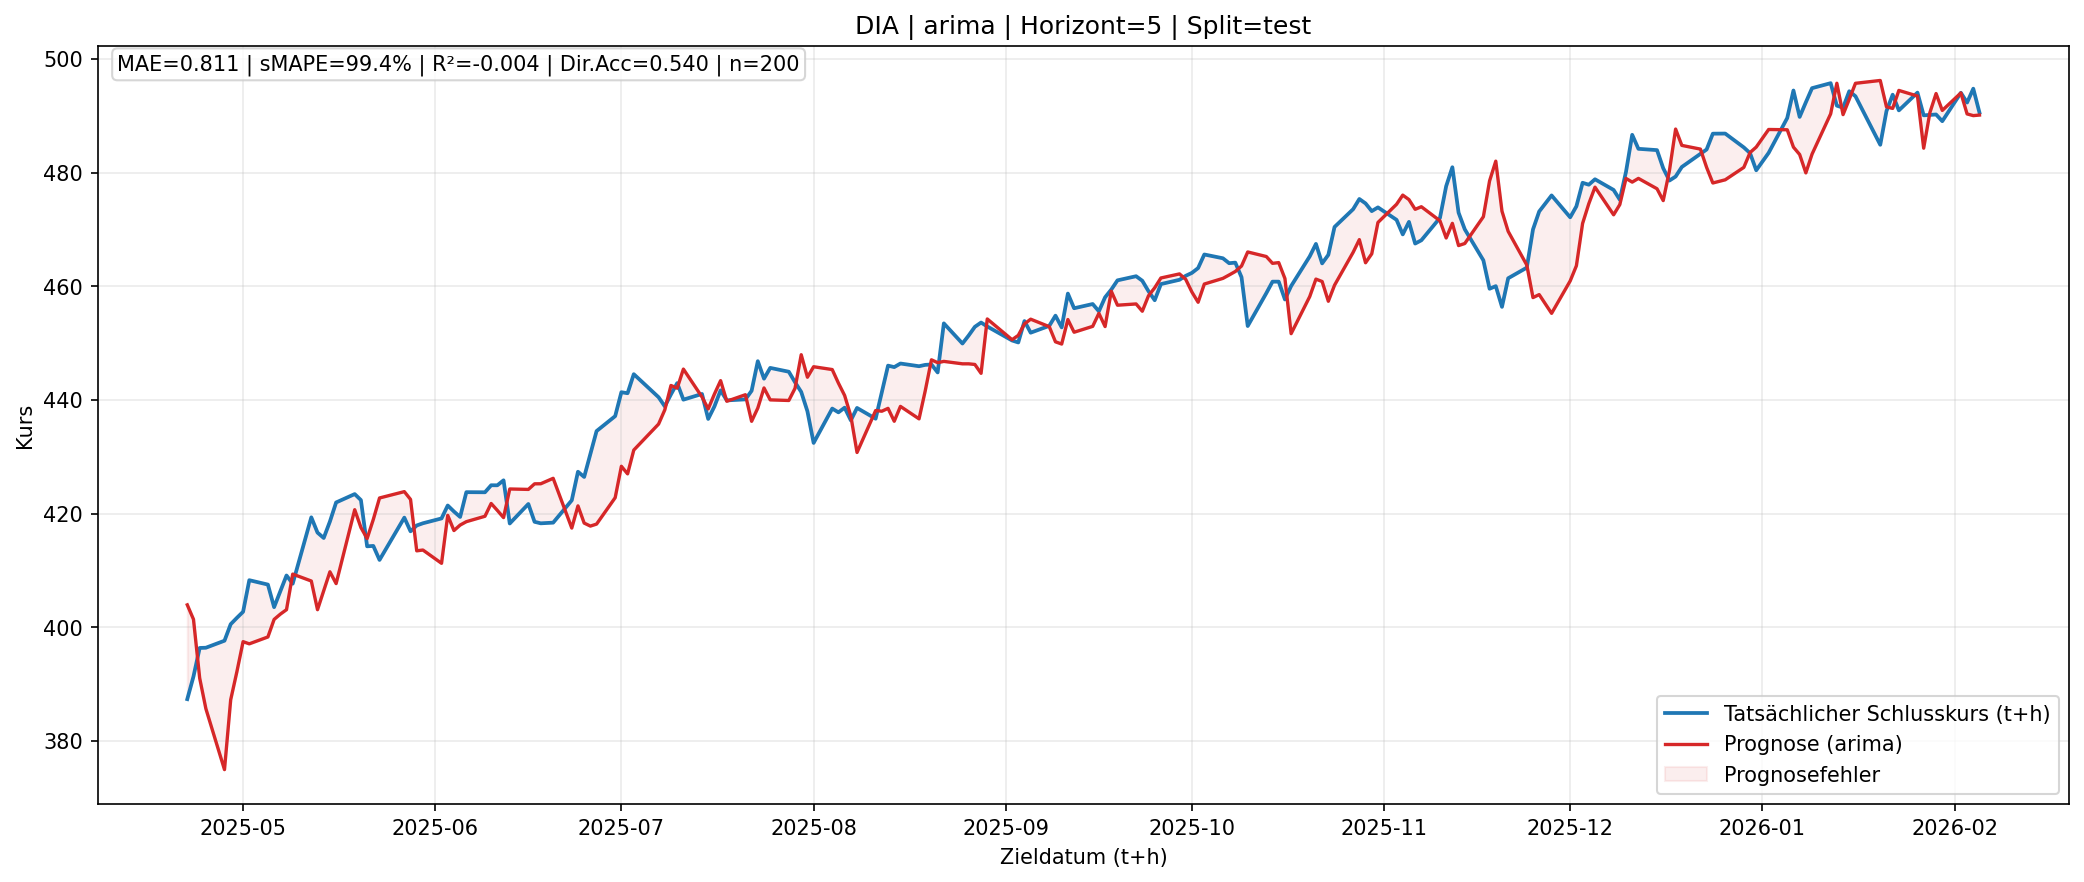
\includegraphics[width=\textwidth]{images/regression}
    \caption{ARIMA-Prognose vs. tatsächlicher Kurs ($h=5$, Testabschnitt)}
    \label{fig:regression}
\end{figure}

\paragraph{Overfitting}

Ein naheliegender Erklärungsansatz ist \textit{Overfitting}. Vergleicht man Validierungs-$R^2$ und Test-$R^2$, bricht die Ridge Regression zwischen beiden Abschnitten besonders stark ein. Der Random Forest ist etwas stabiler, kommt jedoch ebenfalls nicht über negative $R^2$-Werte im Testabschnitt hinaus. Bei über 50 generierten Features und nur ca. 1.400 Trainingsbeobachtungen ist das Verhältnis strukturell ungünstig. Dazu kommt, dass die volatilitätsskalierten Log-Renditen als Zielgröße von Natur aus schwer vorherzusagen sind, was jedoch so beabsichtigt war, um einen realistischen Evaluierungsrahmen zu schaffen.

\subsubsection{Klassifikationsergebnisse}

\begin{table}[ht]
\centering
\caption{Klassifikationsmetriken aus dem Testset ($h = 5$ Handelstage)}
\label{tab:classification_h5}

\begin{tabularx}{\linewidth}{llRRRRR}
\toprule
\textbf{Ticker} & \textbf{Modell} & \textbf{Accuracy} & \textbf{F1} & \textbf{ROC-AUC} & \textbf{Coverage} & \textbf{Uplift} \\
\midrule
  \multirow{3}{*}{\textbf{DIA}} & Base Logistic & 0.620 & 0.759 & \textcolor{bestgreen}{\textbf{0.544}} & \textcolor{bestgreen}{\textbf{0.178}} & $+$0.033 \\
   & Meta Logistic & \textcolor{bestgreen}{\textbf{0.818}} & \textcolor{bestgreen}{\textbf{0.900}} & 0.541 & 0.078 & \textcolor{bestgreen}{\textbf{$+$0.231}} \\
   & Baseline-Rate$^\ddagger$ & 0.587 & 0.740 & --- & 1.000 & --- \\
\bottomrule
\end{tabularx}

\smallskip
{\footnotesize
$^\ddagger$\,Baseline-Rate: häufigste Klasse wird stets vorhergesagt. \quad
Uplift\,$=$\,Accuracy\,$-$\,Baseline-Rate. \quad
\textcolor{bestgreen}{\textbf{Grün}}: bestes Modell je Metrik.}
\end{table}

\paragraph{Coverage und Abstentionsverhalten}

Ein grundlegendes Problem der Klassifikationsauswertung ist die geringe Coverage.
Der Basisklassifikator gibt bei drei von vier Tickern für weniger als 2\,\% der Testbeobachtungen überhaupt eine Vorhersage ab und bei QQQ und XLE überhaupt keine. Lediglich DIA bildet mit einer Coverage von ca. 13\,\% eine Ausnahme. Das liegt an der Threshold-Logik: Das Modell findet kaum Beobachtungen, bei denen es eine ausreichend hohe Konfidenz feststellt, und enthält sich daher fast immer. Bei so wenigen Vorhersagen sind die berechneten Metriken statistisch kaum aussagekräftig.

\paragraph{Genauigkeit bei hoher Konfidenz}

Wo der Basisklassifikator doch Vorhersagen trifft, sind die Genauigkeitswerte teilweise überraschend hoch. Allerdings basieren diese Werte oft auf sehr kleinen Stichproben mit wenigen Beobachtungen, weshalb sie nur bedingt interpretierbar sind. Ob ein echtes Signal vorliegt oder ein statistischer Zufall, lässt sich anhand der vorliegenden Datenmenge nicht zuverlässig beurteilen.

\paragraph{Meta- versus Basisklassifikator}
Der Meta-Klassifikator liefert ein gemischtes Bild: Bei SPY schneidet er deutlich schlechter ab als das einfachere Basismodell, während er bei DIA eine höhere Accuracy erzielt. Bei QQQ und XLE trifft der Basisklassifikator gar keine Vorhersagen, sodass kein direkter Vergleich möglich ist. Insgesamt zeigt sich, dass das Stacking der fehlerhaften Regressionssignale aus Ridge und Random Forest (Abschnitt \ref{regression}) die Eingabe nicht zuverlässig verbessert. Stacking funktioniert nur, wenn die gestapelten Modelle zumindest teilweise korrekte Informationen liefern.

Abbildung \ref{fig:classification} verdeutlicht dieses Versagen exemplarisch für DIA. Der Meta-Klassifikator liefert nur für $7{,}8\%$ eine Prognose, obwohl der Ticker einem einigermaßen gleichmäßigen Trend nach oben folgt.

\begin{figure}[H]
    \centering
    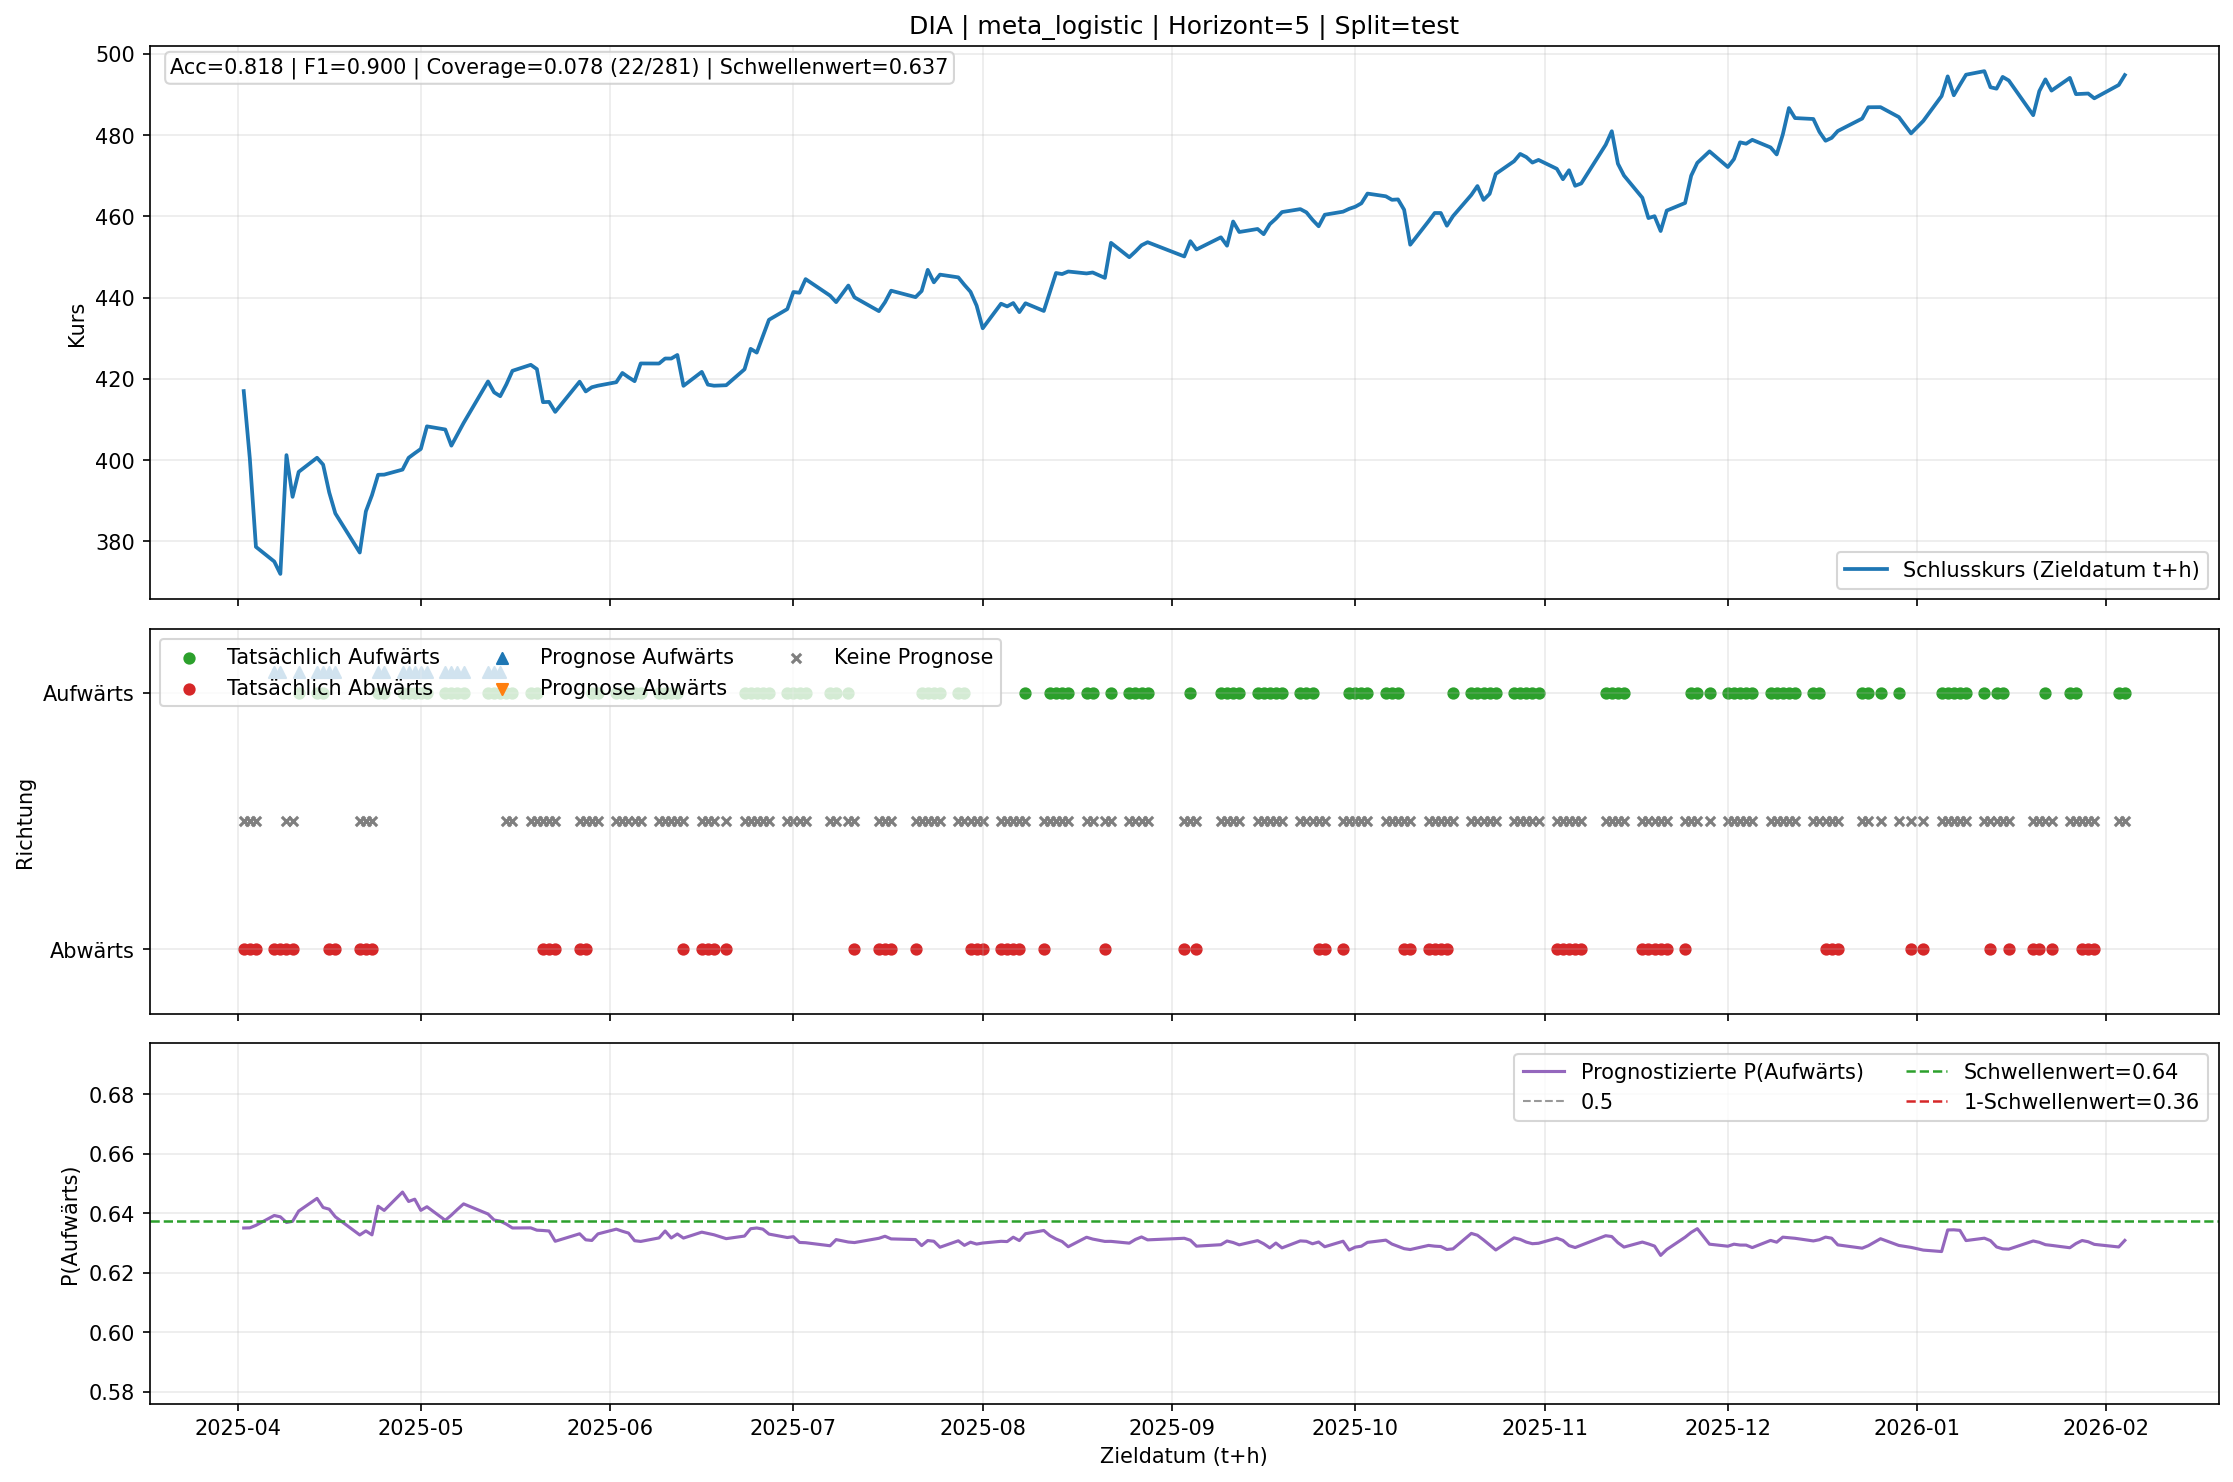
\includegraphics[width=\textwidth]{images/classification}
    \caption{Meta-Klassifikator-Vorhersagen ($h=5$, Testabschnitt).}
    \label{fig:classification}
\end{figure}

\paragraph{Vergleich zur Basisrate}

Kein Modell erzielt gegenüber der Baseline der Mehrheitsklassen einen stabilen positiven Uplift. Bei längeren Prognosehorizonten kommt hinzu, dass Aktienmärkte historisch einen positiven Drift, also mehr Aufwärts- als Abwärtsbewegungen, aufweisen. Ein Modell, das immer „aufwärts" vorhersagt, hat damit schon eine recht hohe nominale Accuracy, ohne irgendetwas gelernt zu haben. Gemessen an dieser Baseline erzielen die Klassifikatoren keinen konsistenten Mehrwert.